\documentclass[aspectratio=169, 10pt]{beamer}\usepackage[]{graphicx}\usepackage[]{color}
% maxwidth is the original width if it is less than linewidth
% otherwise use linewidth (to make sure the graphics do not exceed the margin)
\makeatletter
\def\maxwidth{ %
  \ifdim\Gin@nat@width>\linewidth
    \linewidth
  \else
    \Gin@nat@width
  \fi
}
\makeatother

\definecolor{fgcolor}{rgb}{0.345, 0.345, 0.345}
\newcommand{\hlnum}[1]{\textcolor[rgb]{0.686,0.059,0.569}{#1}}%
\newcommand{\hlstr}[1]{\textcolor[rgb]{0.192,0.494,0.8}{#1}}%
\newcommand{\hlcom}[1]{\textcolor[rgb]{0.678,0.584,0.686}{\textit{#1}}}%
\newcommand{\hlopt}[1]{\textcolor[rgb]{0,0,0}{#1}}%
\newcommand{\hlstd}[1]{\textcolor[rgb]{0.345,0.345,0.345}{#1}}%
\newcommand{\hlkwa}[1]{\textcolor[rgb]{0.161,0.373,0.58}{\textbf{#1}}}%
\newcommand{\hlkwb}[1]{\textcolor[rgb]{0.69,0.353,0.396}{#1}}%
\newcommand{\hlkwc}[1]{\textcolor[rgb]{0.333,0.667,0.333}{#1}}%
\newcommand{\hlkwd}[1]{\textcolor[rgb]{0.737,0.353,0.396}{\textbf{#1}}}%
\let\hlipl\hlkwb

\usepackage{framed}
\makeatletter
\newenvironment{kframe}{%
 \def\at@end@of@kframe{}%
 \ifinner\ifhmode%
  \def\at@end@of@kframe{\end{minipage}}%
  \begin{minipage}{\columnwidth}%
 \fi\fi%
 \def\FrameCommand##1{\hskip\@totalleftmargin \hskip-\fboxsep
 \colorbox{shadecolor}{##1}\hskip-\fboxsep
     % There is no \\@totalrightmargin, so:
     \hskip-\linewidth \hskip-\@totalleftmargin \hskip\columnwidth}%
 \MakeFramed {\advance\hsize-\width
   \@totalleftmargin\z@ \linewidth\hsize
   \@setminipage}}%
 {\par\unskip\endMakeFramed%
 \at@end@of@kframe}
\makeatother

\definecolor{shadecolor}{rgb}{.97, .97, .97}
\definecolor{messagecolor}{rgb}{0, 0, 0}
\definecolor{warningcolor}{rgb}{1, 0, 1}
\definecolor{errorcolor}{rgb}{1, 0, 0}
\newenvironment{knitrout}{}{} % an empty environment to be redefined in TeX

\usepackage{alltt}

% Some important packages
\usepackage{apacite}
\usepackage{epstopdf}
\hypersetup{colorlinks=false, allcolors=purple}
\usepackage{booktabs}
\linespread{1.3}
\usepackage{tabularx}
\usepackage{textpos}  % for the textblock* environment
\usepackage{geometry}
\usepackage{algorithm2e}

% Styles
\usepackage{xcolor}
\definecolor{suffstat}{RGB}{10,159,0}
\definecolor{normconst}{RGB}{87,38,231}

% USC Colors
\definecolor{usccardinal}{RGB}{153,27,30}
\definecolor{uscgold}{RGB}{255,204,0}
\definecolor{usclightgray}{gray}{.7}
\definecolor{uscdarkgray}{gray}{.3}

\usetheme{default}

\setbeamercolor{title}{fg=uscgold, bg=usccardinal}
\setbeamercolor{section in toc}{fg=usccardinal}
\setbeamercolor{frametitle}{use=title, fg=title.fg, bg=title.bg}
\setbeamercolor{item}{fg=uscdarkgray}
\setbeamercolor{normal text}{fg=uscdarkgray}
\setbeamercolor{author in head/foot}{use=title, bg=title.bg, fg=title.fg}
\setbeamercolor{title in head/foot}{use=title, bg=title.bg, fg=title.fg}
\setbeamercolor{author}{use=title, bg=title.bg, fg=title.fg}
\setbeamercolor{date}{use=title, bg=title.bg, fg=title.fg}
\setbeamercolor{institute}{use=title, bg=title.bg, fg=title.fg}
\setbeamercolor{button}{bg=usccardinal, fg=uscgold}


% Figures and tables caption
\setbeamertemplate{caption}{
{\bf\color{usccardinal}\insertcaptionname{} \insertcaptionnumber{}} \insertcaption
}
\setbeamercolor{caption name}{fg=usccardinal}


% Naigation
\makeatother
\setbeamertemplate{footline}
{
  \leavevmode%
  \hbox{%
  \begin{beamercolorbox}[wd=.4\paperwidth,ht=2.25ex,dp=1ex,center]{author in head/foot}%
    \usebeamerfont{author in head/foot}\insertshortauthor
  \end{beamercolorbox}%
  \begin{beamercolorbox}[wd=.6\paperwidth,ht=2.25ex,dp=1ex,center]{title in head/foot}%
    \usebeamerfont{title in head/foot}\insertshorttitle\hspace*{3em}
    \insertframenumber{} / \inserttotalframenumber\hspace*{1ex}
  \end{beamercolorbox}}%
  \vskip0pt%
}
\setbeamertemplate{navigation symbols}{}

\addtobeamertemplate{frametitle}{}{%
\begin{textblock*}{.1\textwidth}(.95\textwidth, -1cm)

\includegraphics[width=1\textwidth]{4-Line_KeckSOMofUSC_CardOnGold1.eps}
\end{textblock*}
}


% Avoid appendix showin in toc -------------------------------------------------
% \nobibintoc
% ------------------------------------------------------------------------------

\title[Stat. Comp. Bioinf \& SocNets.]{Statistical and computational methods for bioinformatics and social network analysis\linebreak{\small or how did I learn to stop worrying and love the bomb}}
\author[GGVY]{George G Vega Yon}
\institute[USC-PREVMED]{University of Southern California, Department of Preventive Medicine}

% Some definitions
\def\cursection{\frame{\frametitle{Contents}\tableofcontents[current]}}
\newcommand{\ergmitopkg}[0]{\texttt{ergmito}}
\newcommand{\aphylopkg}[0]{\texttt{aphylo}}
\graphicspath{{.}{fig/}}


% ------------------------------------------------------------------------------
% ------------------------------------------------------------------------------
% --------------------------- END OF PREAMBLE ----------------------------------
% ------------------------------------------------------------------------------
% ------------------------------------------------------------------------------
\IfFileExists{upquote.sty}{\usepackage{upquote}}{}
\begin{document}
% \SweaveOpts{concordance=TRUE}

% ------------------------------------------------------------------------------
\setbeamercolor{background canvas}{bg=usccardinal}
\begin{frame}[noframenumbering]
\maketitle
\end{frame}
\setbeamercolor{background canvas}{bg=}

% ------------------------------------------------------------------------------
\section{Paper 1: Exponential Random Graph Models for Small Networks}
\frame{\frametitle{Contents}\tableofcontents}
\cursection

\begin{frame}
\frametitle{What are Exponential Random Graph Models}

Exponential Family Random Graph Models, aka ERGMs are:\pause

\begin{itemize}[<+->]
\item Statistical models of (social) networks
\item In simple terms: statistical inference on what network patterns/structures/motifs
govern the data-generating process\pause
\begin{figure}
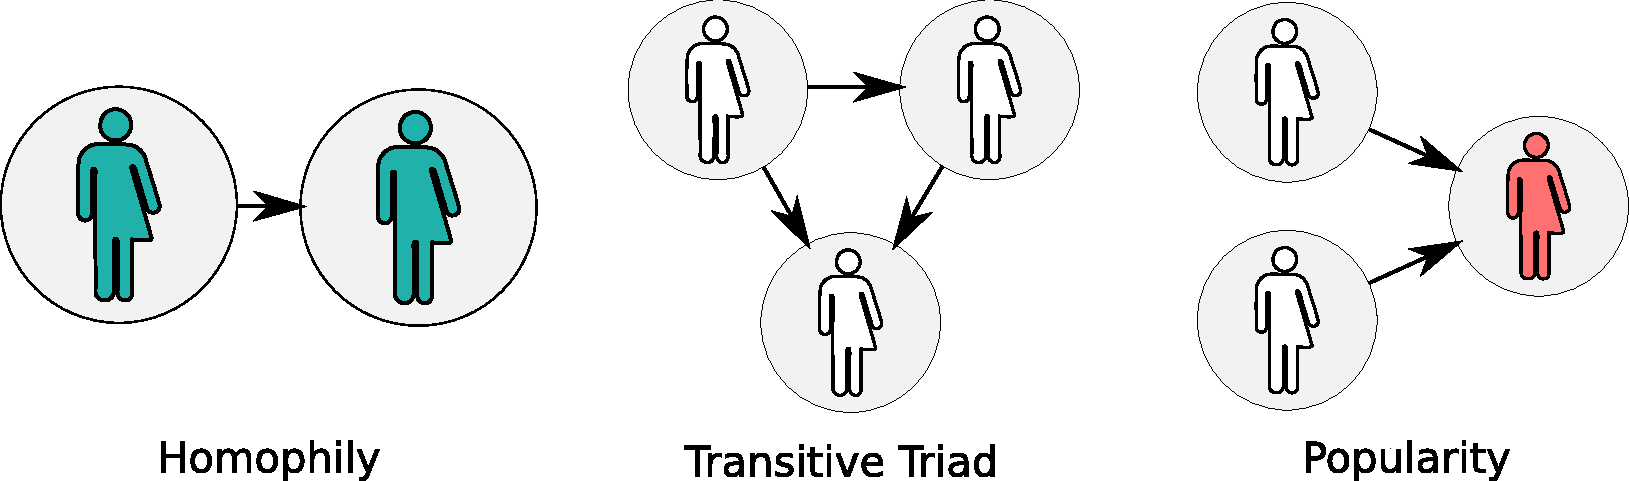
\includegraphics[width=.6\linewidth]{friendly-terms.pdf}
\end{figure}
\end{itemize}

\end{frame}

% ------------------------------------------------------------------------------
\begin{frame}[label=ergmeq]
\frametitle{ERGMs (cont'd)}
\centering
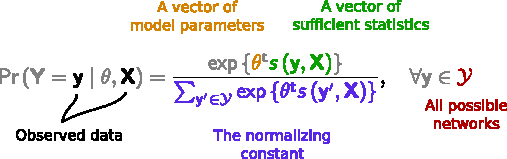
\includegraphics[width=.7\linewidth]{parts-of-ergm.pdf}
\end{frame}

\hyperlink{ergmterms}{\beamergotobutton{more on terms}}

% ------------------------------------------------------------------------------
\begin{frame}[label=art]
\frametitle{ERGMs: State of the Art}
\pause
Small-large (dozens to a couple of thousand vertices) networks

\begin{itemize}
\item Markov Chain Monte Carlo (MCMC) based approaches like MC-MLE or Robbins-Monro Stochastic approximation. \hyperlink{mcmle}{\beamergotobutton{details}}
\item Maximum Pseudo Likelihood (MPLE)
\end{itemize}\pause

large-huge networks (up to the millions of vertices)

\begin{itemize}
\item Semi-parametric bootstrap
\item Conditional joint estimation (like snowball sampling, a.k.a. divide and conquer)
\item Equilibrium Expectation Algorithm (millions of vertices)
\end{itemize}\pause

What about tiny to small networks?

\end{frame}

% ------------------------------------------------------------------------------
\begin{frame}
\frametitle{A frame with examples of small networks...}
\begin{figure}
\centering

\includegraphics[width=.6\linewidth]{american-chopper-argument-ergmitos.png}
\end{figure}
\end{frame}

% ------------------------------------------------------------------------------
\begin{frame}
\frametitle{ERGMs for small networks}

MC-MLE works great (we have some simulations showing this), but it has some
problems:\pause

\begin{itemize}[<+->]
\item Possible accuracy issues (error rates)
\item Prone to degeneracy problems (sampling and existance of MLE)
\item It is not MLE,
\end{itemize}

What shall we do then?

\end{frame}

% ------------------------------------------------------------------------------
\begin{frame}[label=ergmito]
\frametitle{ERGMs for Small Networks}

\pause
\begin{itemize}[<+->]
\item In the case of small-enough networks, computation of the likelihood becomes
computationally feasible.
\item For example, a network with 5 nodes has 1,048,576
unique configurations.
\item This allow us to directly compute {\bf\color{normconst} the normalizing constant}.
\item Using the exact likelihood opens a huge window of methodological-possibilities.
\end{itemize}\pause
We implemented this and more in the \ergmitopkg{} R package \hyperlink{ergmitopkg}{\beamergotobutton{more}}
\end{frame}

% ------------------------------------------------------------------------------
\begin{frame}
\frametitle{Paper 1 Simulation Studies}

In order to compare the MLE with the MC-MLE estimation method, we performed a simulation study with the following features:\pause

\begin{itemize}[<+->]
\item Draw 20,000 samples of groups of small networks
\item Each group had prescribed: (model parameters, number of networks, sizes of the networks)
\item Each group could have from 5 to 300 small networks
\item We estimated the models using MC-MLE and MLE.
\end{itemize}

\end{frame}

% ------------------------------------------------------------------------------
\begin{frame}
\frametitle{Paper 1 Simulation Studies: Empirical Type I error}

\footnotesize

\begin{table}[ht]
	\centering
	\begin{tabular}{ccccc}
		\toprule & & \multicolumn{2}{c}{P(Type I error)} \\ \cmidrule(r){3-4}
		Sample size & N. Simulations & MC-MLE & MLE & chi2 \\ 
		\midrule
		5 & 2,189 & 0.084 & 0.057 & 11.71 *** \\ 
		10 & 2,330 & 0.070 & 0.045 & 12.46 *** \\ 
		15 & 2,395 & 0.084 & 0.066 & 5.55 * \\ 
		20 & 2,430 & 0.074 & 0.060 & 3.58  \\ 
		30 & 2,460 & 0.057 & 0.052 & 0.67  \\ 
		50 & 2,495 & 0.046 & 0.044 & 0.17  \\ 
		100 & 2,499 & 0.048 & 0.048 & 0.00  \\ 
		\bottomrule
	\end{tabular}
	\caption{\label{tab:typeI}Empirical Type I error rates. The $\chi^2$ statistic is from a 2-sample test for equality of proportions, and the significance levels are given by *** $p < 0.001$, ** $p < 0.01$, and * $p < 0.05$. The lack of fitted samples in some levels is due to failure of the estimation method.} 
\end{table}

\end{frame}

% ------------------------------------------------------------------------------
\begin{frame}[label=ergmitoexperiment]
\frametitle{Paper 1 Simulation Studies: Elapsed time}

\begin{figure}
\centering
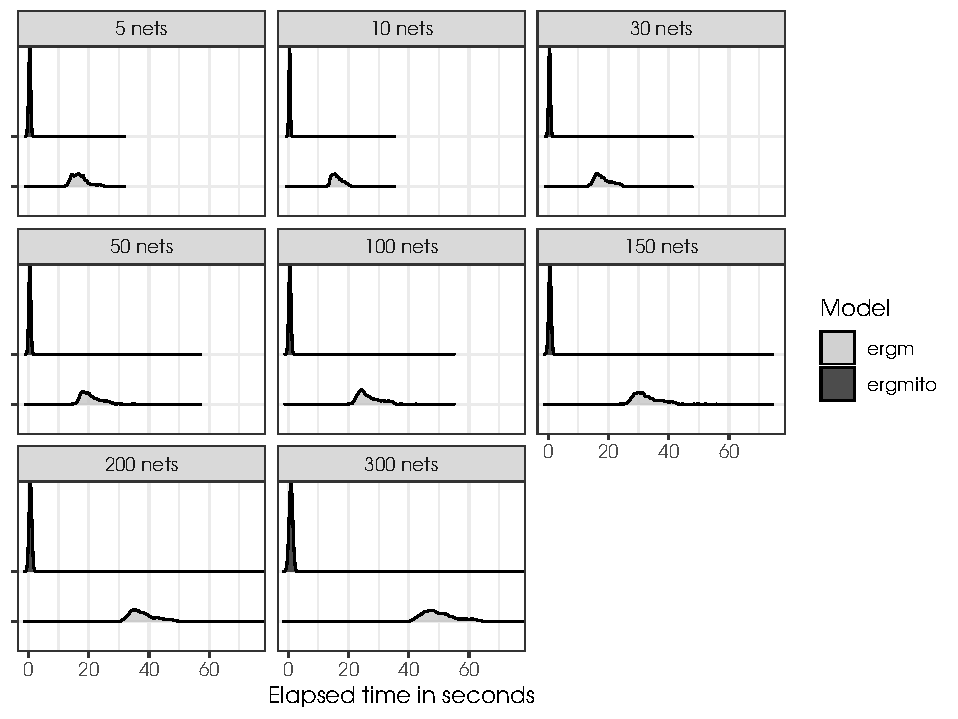
\includegraphics[width=.6\linewidth]{bias-elapsed-02-various-sizes-4-5-ttriad.pdf}
\end{figure}

\hyperlink{ergmsims}{\beamergotobutton{more results}}

\end{frame}

% ------------------------------------------------------------------------------
\begin{frame}
\frametitle{Paper 1: Key takeaway}
\pause
\begin{itemize}[<+->]
\item Developed a new extension of ERGMs using exact statistics for small networks
(families, teams, ego-centered, etc.)
\item Performance: Same (un)bias, Lower Type I error rates, (way) faster.
\item Opens the door the new methods.
\end{itemize}
\end{frame}


% ------------------------------------------------------------------------------
\section{Paper 2: On the prediction of gene functions using phylogenetic trees}
\cursection

\begin{frame}
\frametitle{Phylogenetic Trees}
\pause
\begin{itemize}[<+->]
\item It can be very general: think of the tree of life
\item Nowadays, thanks to gene-sequencing techniques, we are building trees at the
gene level (using sequence-alignment methods, i.e. comparing gene sequences to see how much similar/different two genes are between and within species (whattt!)).
\item A single phylogenetic tree can host multiple species
\end{itemize}

\end{frame}

% ------------------------------------------------------------------------------
\begin{frame}

\begin{knitrout}
\definecolor{shadecolor}{rgb}{0.969, 0.969, 0.969}\color{fgcolor}

{\centering 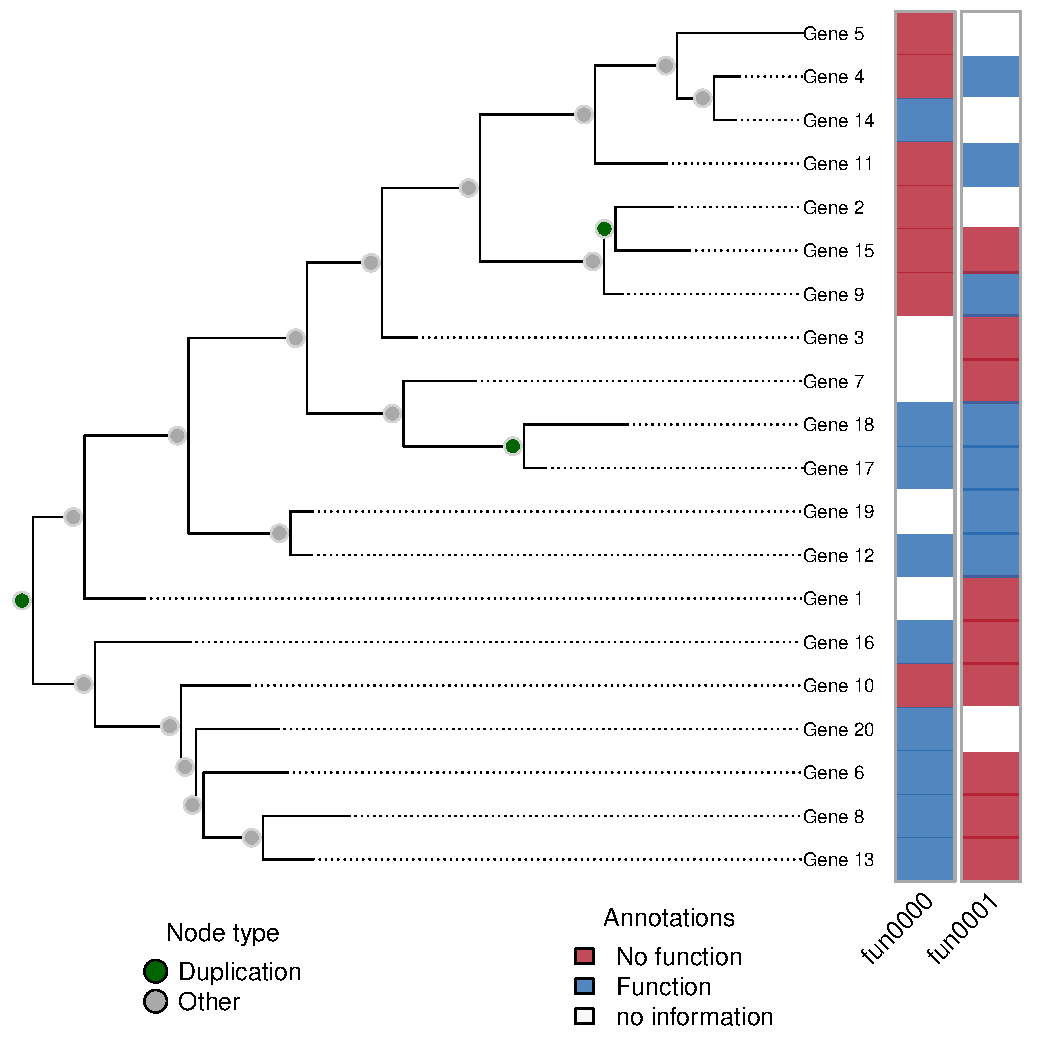
\includegraphics[width=.6\linewidth]{figure/random-tree-1} 

}



\end{knitrout}


\end{frame}

\begin{frame}
\frametitle{Gene Functional Annotations: The Gene Ontology Project}

% ------------------------------------------------------------------------------
\begin{table}
\footnotesize
\begin{tabular}{lm{.6\linewidth}}
\toprule
\textbf{Accession} & GO:0060047 \\
\textbf{Name} & heart contraction \\
\textbf{Ontology} & biological\_process \\
\textbf{Synonyms} & heart beating, cardiac contraction, hemolymph circulation \\
\textbf{Alternate} & IDs None \\
\textbf{Definition} & The multicellular organismal process in which the heart decreases in volume in a 
characteristic way to propel blood through the body. Source: GOC:dph \\
\bottomrule
\end{tabular}
\caption{Heart Contraction Function. source: \href{http://amigo.geneontology.org/amigo/term/GO:0060047}{amigo.geneontology.org}}
\end{table}

\def\tmpwidth{.15\linewidth}
\begin{table}
\footnotesize
\begin{tabular}{*{4}{p{\tmpwidth}<\centering}}
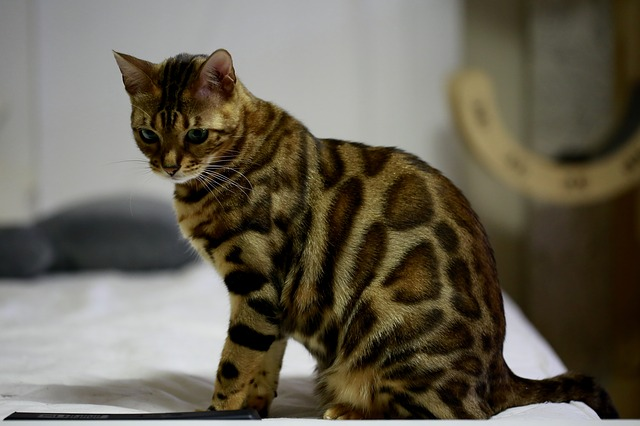
\includegraphics[width=1\linewidth]{cat.jpg} \linebreak pthr10037 & %
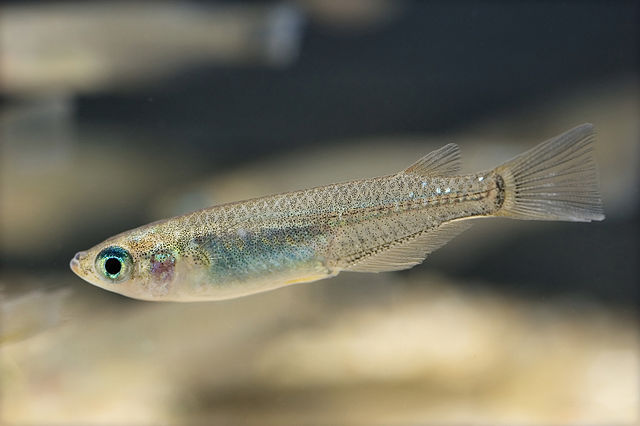
\includegraphics[width=1\linewidth]{Oryzias_latipes.jpg} \linebreak \textbf{pthr11521} & %
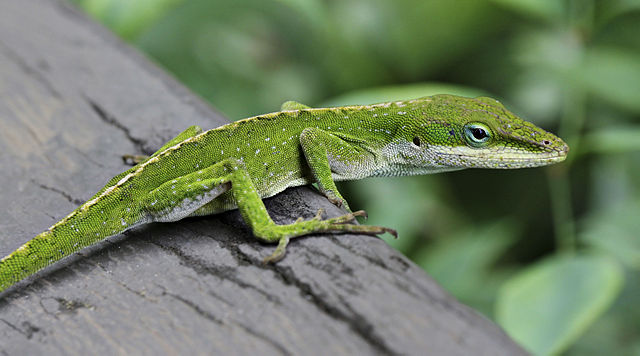
\includegraphics[width=1\linewidth]{Anole_Lizard.jpg} \linebreak \textbf{pthr11521} & %
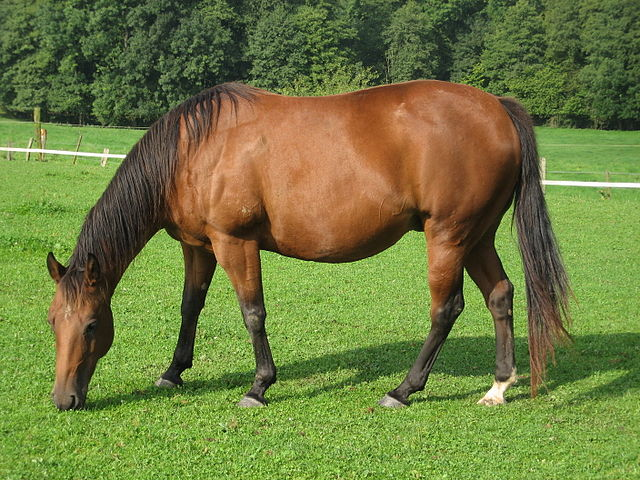
\includegraphics[width=1\linewidth]{horse.jpg} \linebreak pthr24356
\end{tabular}
\end{table}


\end{frame}

\begin{frame}
\frametitle{Speciation}
\begin{figure}
\centering
\def\svgwidth{.8\linewidth}
\tiny
% Source 
\input{fig/Drosophila_speciation_experiment.pdf_tex}
\caption{\citeA{Dodd1989}: After one year of isolation, flies showed a significant level or assortativity in mating (\href{https://commons.wikimedia.org/wiki/File:Drosophila_speciation_experiment.svg}{wikimedia})}
\end{figure}
\end{frame}

\begin{frame}
\frametitle{Duplication}
\begin{figure}
\centering
\def\svgwidth{.6\linewidth}
\tiny
% Source : https://en.wikipedia.org/wiki/File:Evolution_fate_duplicate_genes_-_vector.svg
\input{fig/Evolution_fate_duplicate_genes_-_vector.pdf_tex}
\caption{A key part of molecular innovation, gene duplication provides opportunity for new functions to emerge (\href{https://en.wikipedia.org/wiki/File:Evolution_fate_duplicate_genes_-_vector.svg}{wikimedia})}
\end{figure}
\end{frame}

% ------------------------------------------------------------------------------
\begin{frame}
\frametitle{An evolutionary model of gene functions (algorithmic view)}

\footnotesize

\begin{algorithm}[H]
\SetAlgoLined
\KwData{A phylogenetic tree, $\{\pi, \mu, \psi\}$(Model probabilities)}
\KwResult{An annotated tree}
\pause
\For{$n \in PostOrder(N)$}{
  $\mbox{\bf\color{usccardinal}Nodes gain/loss function depending on their parent}$\;\pause
  \Switch{class of $n$}{
    \uCase{root node}{
      Gain function with probability $\pi$\;
    }\pause
    \uCase{interior node} {\pause
      \lIf{Parent has the function}{Keep it with prob. $(1-\mu_1)$}\pause
      \lElse{Gain it with prob. $\mu_0$}\pause
    }
  }\pause
  $\mbox{\bf\color{usccardinal}Finally, we allow for mislabeling}$\;\pause
  \uIf{$n$ is leaf}{\pause
    \lIf{has the function}{Mislabel with prob. $\psi_1$}\pause
    \lElse{Mislabel with prob. $\psi_0$}\pause
  }
}
\end{algorithm}

\normalsize

% 
% The general points of the model
% \begin{itemize}[<+->]
% \item The rootnode in a phylogenetic tree is the best idea we have about the past, meaning,
% it could be that the tree has more behind, i.e. so functions may be gained since the beginning.
% \item At each step in evolution (interior node), there is a probability that the gene may
% gain/loss the function.
% \item Those probabilities vary depending on the type of the node: We belive that functional
% changes may happen at Duplication nodes.
% \end{itemize}
\end{frame}

% ------------------------------------------------------------------------------
\begin{frame}
\frametitle{An evolutionary model of gene functions: Formal statement}

\begin{itemize}[<+->]
\item The whole is based on the markov-assumption: The current state of the gene can be
fully explained by its parent(s).

\item For this we use Felsensteins' pruning algorithm (also known as...)

Formally

$$
P(x = 1) = P(x = 1| x_p = 0)P(\mbox{Gain}) + P(x = 1| x_p = 1)P(\mbox{No loss})
$$
\end{itemize}

\end{frame}

% ------------------------------------------------------------------------------
\begin{frame}
\frametitle{Paper 2: Estimation of the model}
The model has (so far) 7 fixed parameters
\begin{description}
\item[$\psi_0, \psi_1$] Probability of making a mistake (mislabel)
\item[$\mu_{d0}, \mu_{d1}$] Probability of functional gain/loss (duplication nodes)
\item[$\mu_{s0}, \mu_{s1}$] Probability of functional gain/loss (other nodes)
\item[$\pi$] Probability that the root has the function
\end{description}
\end{frame}

% ------------------------------------------------------------------------------
\begin{frame}[label=aphylo]
\frametitle{Paper 2: Estimation of the model (cont'd)}
\begin{itemize}
\item We developed a full set of tools (C++ library + R pacakge) for this framework
\hyperlink{aphylopkg}{\beamergotobutton{more}}
\item Estimation is done via: MLE, MAP, and MCMC (using an adaptive kernel)
\item Posterior probabilities are estimated using the conditional on the observed data.
\item To evaluate performance, we used two datasets: manually (fully) annotated (inferred) trees, and experimentally annotated trees
\end{itemize}
\end{frame}

% ------------------------------------------------------------------------------
\begin{frame}
\frametitle{Paper 2: Pooled estimation}

\begin{table}[ht]
\centering
\scalebox{0.6}{
\begin{tabular}{l*{8}{m{0.14\linewidth}}}
  \toprule
 & (1) & (2) & (3) & (4) & (5) & (6) & (7) & (8) \\ 
  \midrule
$\psi_0$ & 0.00 & 0.00 & 0.23 & 0.25 & 0.00 & 0.00 & 0.21 & 0.25 \\ 
  $\psi_1$ & 0.00 & 0.00 & 0.01 & 0.01 & 0.00 & 0.00 & 0.00 & 0.01 \\ 
  $\mu_{d0}$ & 0.01 & 0.01 & 0.97 & 0.96 & 1.00 & 0.01 & 1.00 & 0.98 \\ 
  $\mu_{d1}$ & 0.01 & 0.02 & 0.52 & 0.58 & 0.25 & 0.02 & 0.51 & 0.58 \\ 
  $\mu_{s0}$ & 0.00 & 0.00 & 0.05 & 0.06 & 0.07 & 0.00 & 0.05 & 0.06 \\ 
  $\mu_{s1}$ & 0.01 & 0.01 & 0.01 & 0.02 & 0.01 & 0.01 & 0.01 & 0.02 \\ 
  $\pi$ & 0.81 & 0.91 & 0.78 & 0.45 & 0.82 & 0.91 & 0.83 & 0.49 \\ 
  Tree count & 88 & 88 & 141 & 141 & 88 & 88 & 141 & 141 \\ 
\midrule   Method & MCMC & MCMC & MCMC & MCMC & MLE & MLE & MLE & MLE \\ 
  Prior & Uniform & Beta & Uniform & Beta & Uniform & Beta & Uniform & Beta \\ 
  Inferred & Yes & Yes & No & No & Yes & Yes & No & No \\ 
  AUC & 1.00 & 1.00 & 0.69 & 0.67 & 0.98 & 1.00 & 0.70 & 0.67 \\ 
  P. Score (obs) & 1.00 & 1.00 & 0.81 & 0.81 & 0.92 & 1.00 & 0.81 & 0.81 \\ 
  P. Score (random) & 0.71 & 0.71 & 0.61 & 0.61 & 0.71 & 0.71 & 0.61 & 0.61 \\ 
   \bottomrule
\end{tabular}
}
\caption{Parameter estimates using different estimation methods, priors, and types of annotations.} 
\end{table}

\end{frame}

% ------------------------------------------------------------------------------
\begin{frame}
\frametitle{Paper 2: Pooled estimation (worth it?)}

\begin{figure}
\centering
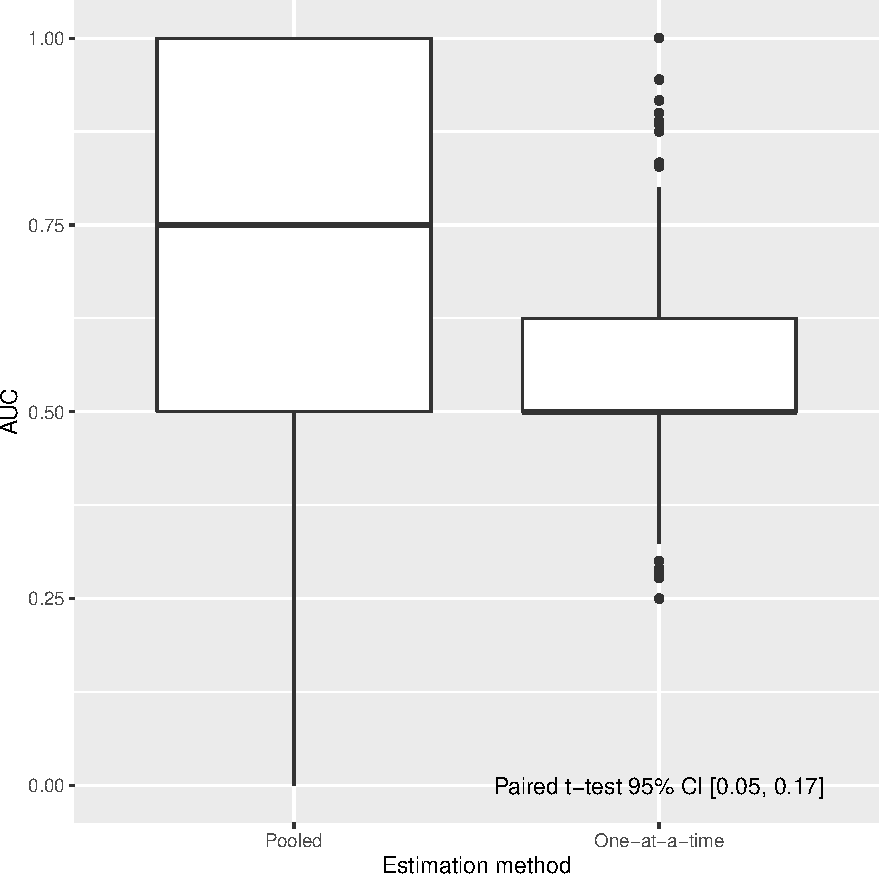
\includegraphics[width=.5\linewidth]{comparing-accuracy-1.pdf}
\end{figure}

\end{frame}

% ------------------------------------------------------------------------------
\begin{frame}
\frametitle{Paper 2: Leave-one-out predictions}

\begin{figure}
\centering
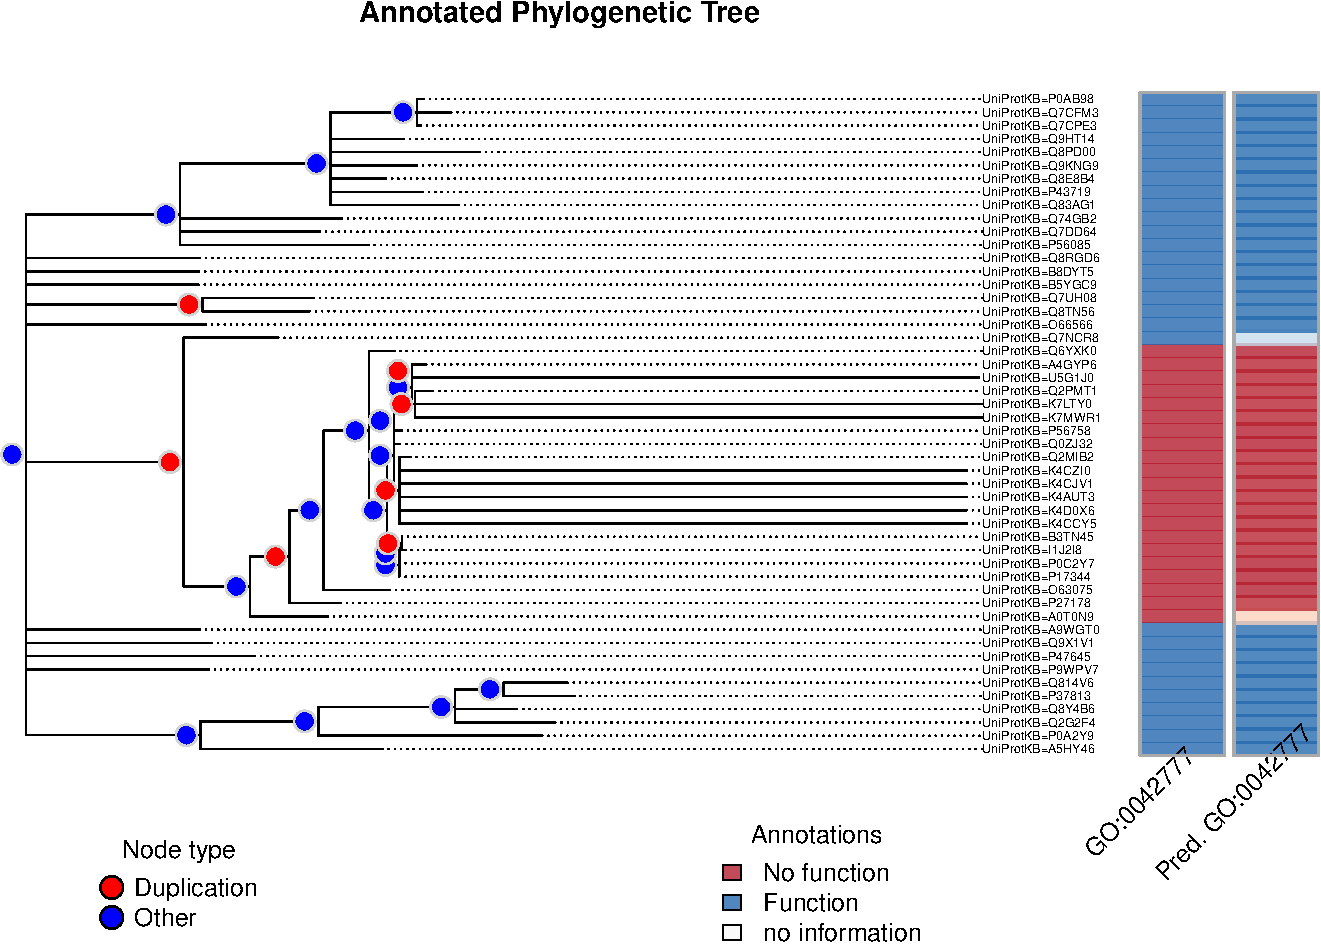
\includegraphics[width=.7\linewidth]{annotations1.pdf}
\end{figure}

\end{frame}

% ------------------------------------------------------------------------------
\begin{frame}
\frametitle{Paper 2: Out-of-sample-predictions}

\begin{figure}
\centering
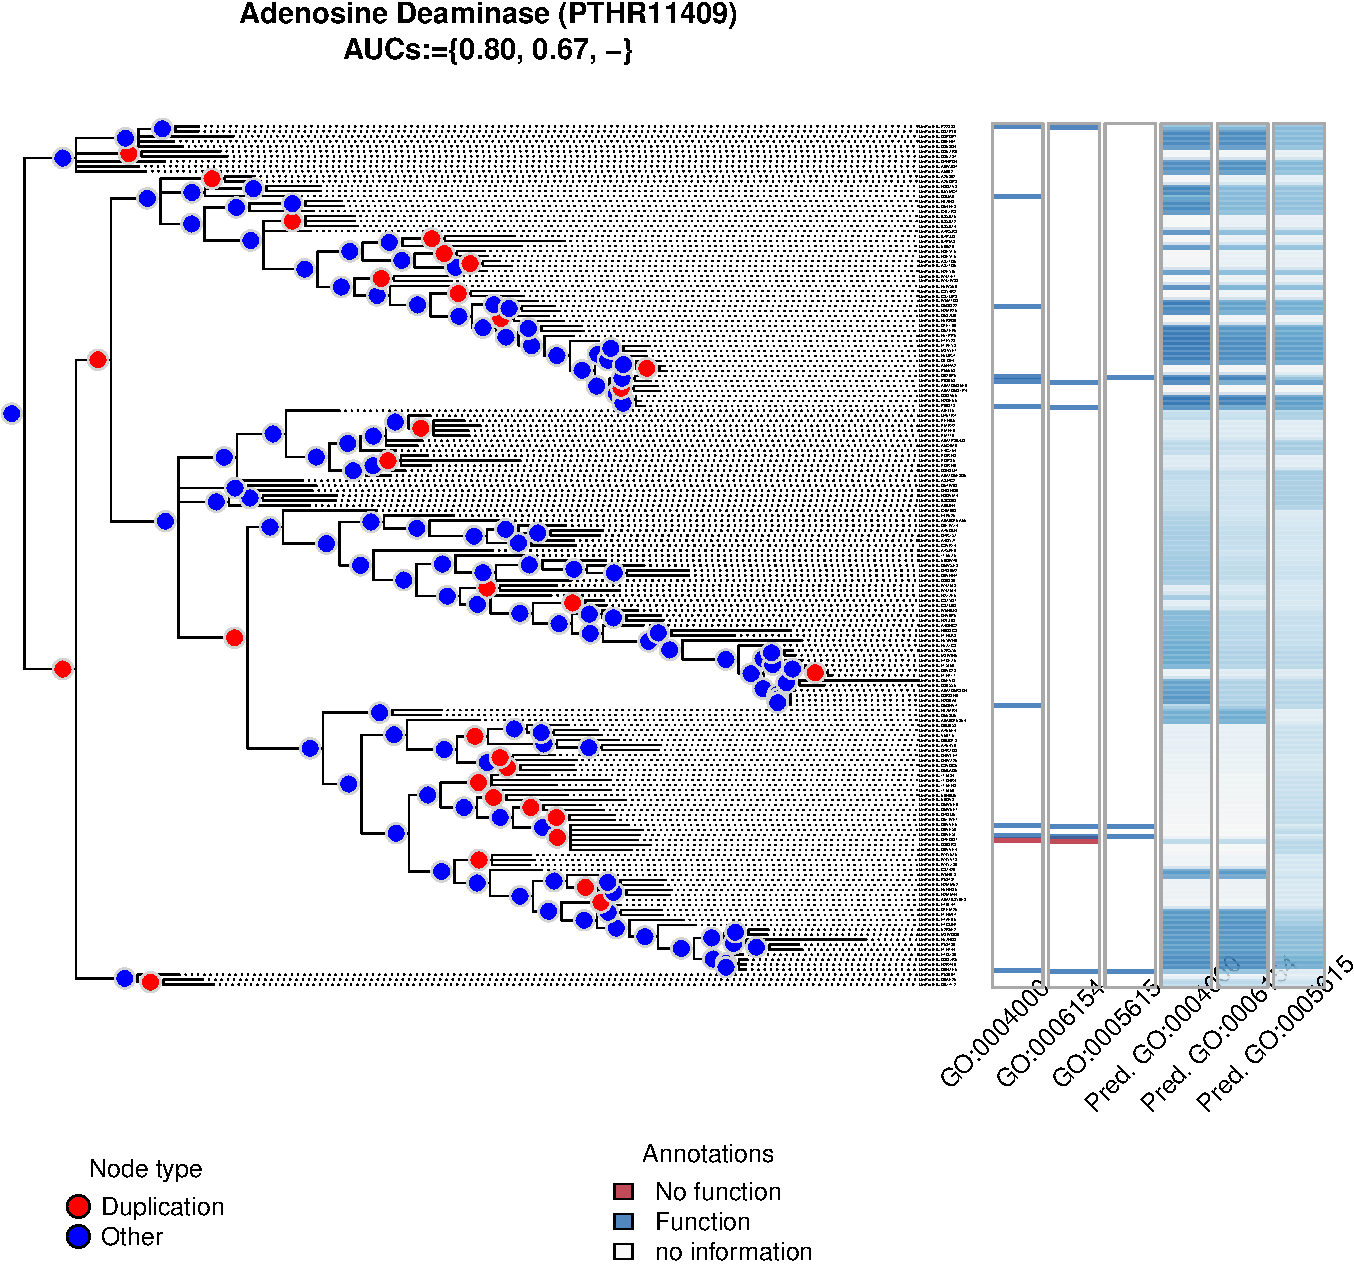
\includegraphics[width=.65\linewidth]{out-of-sample1-1.pdf}
\end{figure}

\end{frame}

% ------------------------------------------------------------------------------
\begin{frame}
\frametitle{Paper 2: Key takeaways}
\pause
\begin{itemize}[<+->]
\item (Yet another) model for predicting gene functions using phylogenetics
\item Big difference... computationally scalable
\item Meaningful biological results
\item Preliminary accuracy results comparable to state-of-the-art phylo-based
models
\end{itemize}
\end{frame}

% ------------------------------------------------------------------------------
\section{Future directions}
\begin{frame}
\frametitle{Future directions: ERGMitos}

Possible venues to continue\pause

\begin{itemize}[<+->]
\item Identify an adequate test for goodness-of-fit assesment
\item Extend to estimation of large graphs by splitting the networks in induced-subgraphs
\end{itemize}

\end{frame}

\begin{frame}
\frametitle{Future directions: Gene functional prediction}

Possible venues to continue\pause

\begin{itemize}[<+->]
\item Incorporate more external information using leaf(and node?) level features.
\item Adapt the model to incorporate joint estimation of functions using pseudo-likelihood.

$$
P(a, b, c) \approx P(a,b)P(b,c)P(a,c)
$$
\item Make the model hierarchical when pooling trees: different mutation rates.
\end{itemize}

\end{frame}


% ------------------------------------------------------------------------------
\section{Things that are very interesting but I most probably won't have any time to discuss with the attendees}

\begin{frame}
Here are some by-products of my research here at USC

\begin{itemize}
\item The slurmR R package
\item The pruner C++ library
\item The fmcmc R package
\end{itemize}

\end{frame}

\renewcommand{\section}[2]{}%
\appendix
\begin{frame}[allowframebreaks]
\frametitle{References}
\bibliographystyle{apacite}
\bibliography{bibliography.bib}
\end{frame}


% ------------------------------------------------------------------------------
% ------------------------------------------------------------------------------
% ------------------------------------------------------------------------------
% ------------------------------------------------------------------------------
% ------------------------------------------------------------------------------

\begin{frame}[label=ergmterms]

{\bf\color{suffstat} Sufficient statistics} have various forms

\def\fig1width{.45\linewidth}
\begin{figure}[tb]
\centering
\begin{tabular}{m{.2\linewidth}<\centering m{.4\linewidth}<\raggedright}
\toprule Representation & Description  \\ \midrule

\includegraphics[width=\fig1width]{ergm-terms/mutual.pdf} & Mutual Ties (Reciprocity)\linebreak[4]$\sum_{i\neq j}y_{ij}y_{ji}$  \\
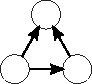
\includegraphics[width=\fig1width]{ergm-terms/ttriad.pdf} & Transitive Triad (Balance)\linebreak[4]$\sum_{i\neq j\neq k}y_{ij}y_{jk}y_{ik}$  \\

\includegraphics[width=\fig1width]{ergm-terms/homophily.pdf} & Homophily\linebreak[4]$\sum_{i\neq j}y_{ij}\mathbf{1}\left(x_i=x_j\right)$ \\
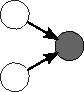
\includegraphics[width=\fig1width]{ergm-terms/nodeicov.pdf} & Covariate Effect for Incoming Ties\linebreak[4]$\sum_{i\neq j}y_{ij}x_j$ \\
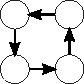
\includegraphics[width=\fig1width]{ergm-terms/fourcycle.pdf} & Four Cycle\linebreak[4]$\sum_{i\neq j \neq k \neq l}y_{ij}y_{jk}y_{kl}y_{li}$  \\
\bottomrule
\end{tabular}
\end{figure}

\hyperlink{ergmeq}{\beamerreturnbutton{go back}}
\end{frame}

% ------------------------------------------------------------------------------
\begin{frame}[label=mcmle]
\frametitle{ERGMs: The MC-MLE approach}

One of the most popular methods for estimating ERGMs is the MC-MLE approach (citations here)

This consists on the folling steps

\begin{enumerate}
\item Start from a sensible guess on what should be the population parameters
(usually done using pseudo-MLE esimtation)
\item While the algorithm doesn't converge, do:
  \begin{enumerate}
  \item Simulate a stream of networks with the current state of the parameter,
  $\theta_t$
  \item Using the law of large numbers, approximate the ratio of likelihoods 
  based on the parameter $\theta_t$, this is the objective function
  \item Update the parameter by a Newton-Raphson step
  \item Next iteration
  \end{enumerate}
\end{enumerate}

\hyperlink{art}{\beamerreturnbutton{go back}}


\end{frame}

% ------------------------------------------------------------------------------
\begin{frame}[label=ergmitopkg]
\frametitle{The \ergmitopkg{}}

\begin{itemize}
\item Implements estimation of ERGMs using exact statistics for small networks
\item Metaprogramming allows specifying likelihood (and gradient) functions for
joint models
\item Includes tools for simulating, and postestimation checks
\item Getting ready for CRAN!
\end{itemize}

\hyperlink{ergmito}{\beamerreturnbutton{go back}}

\end{frame}

% ------------------------------------------------------------------------------
\begin{frame}[label=ergmsims,allowframebreaks]
\frametitle{Paper 1 Simulation Studies: Error rate}

\begin{figure}
\centering
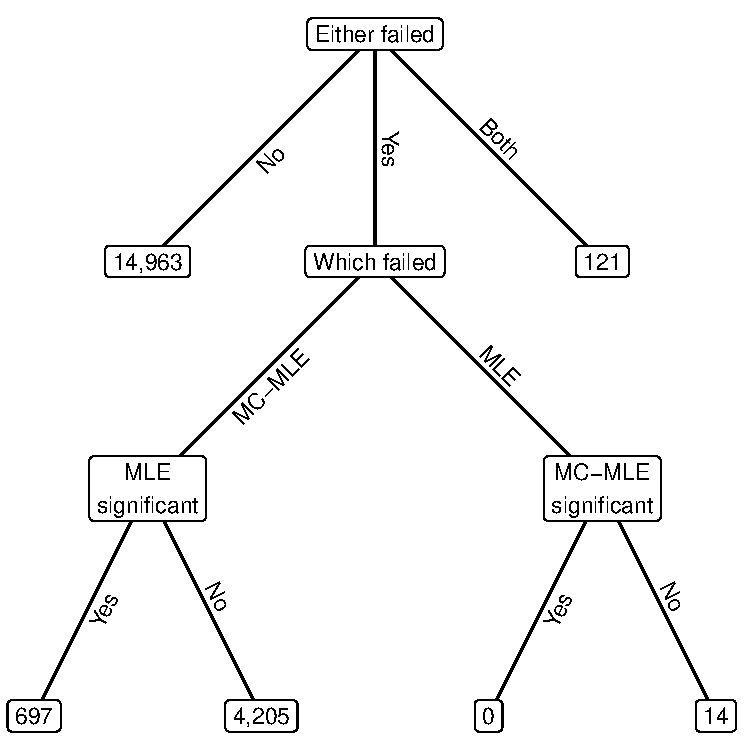
\includegraphics[width=.4\linewidth]{failed-tree.pdf}
\end{figure}

\hyperlink{ergmitoexperiment}{\beamerreturnbutton{go back}}

\end{frame}

\begin{frame}
\frametitle{Paper 1 Simulation Studies: Empirical Bias}

\begin{figure}
\centering
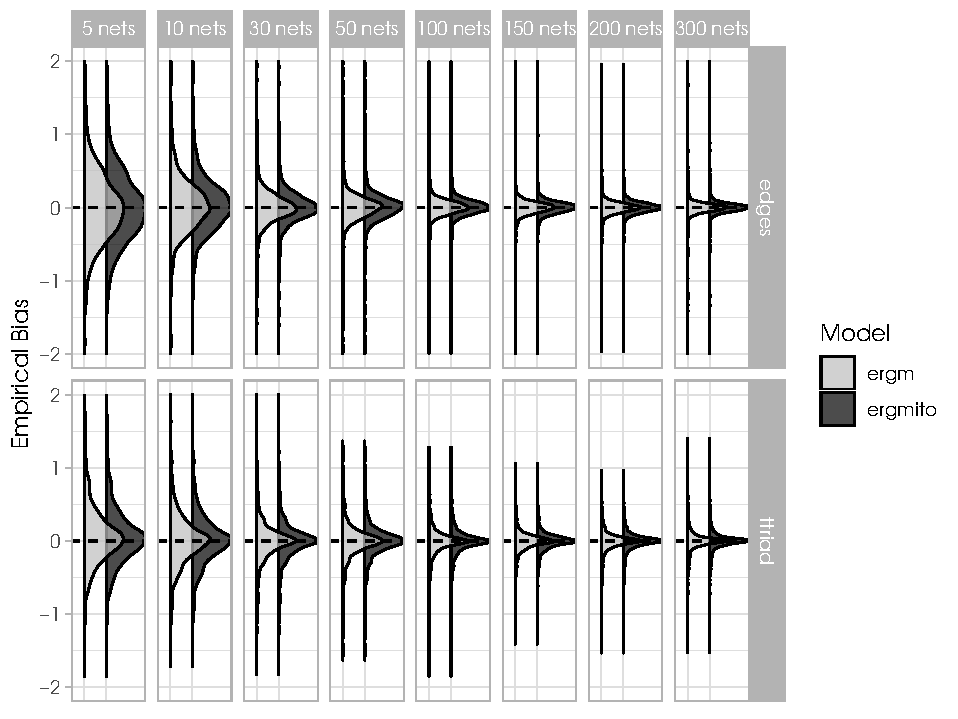
\includegraphics[width=.6\linewidth]{bias-02-various-sizes-4-5-ttriad.pdf}
\end{figure}

\hyperlink{ergmitoexperiment}{\beamerreturnbutton{go back}}

\end{frame}

% ------------------------------------------------------------------------------
\begin{frame}[label=aphylopkg]
\frametitle{The \aphylopkg{}}

\begin{itemize}
\item TBF
\end{itemize}

\hyperlink{aphylo}{\beamerreturnbutton{go back}}
\end{frame}

\end{document}

